\section{La panadería}

\subsection{Presentación del caso}

Gestionamos una panadería artesana en Miraflores de la Sierra. En nuestra panadería se fabrican tres tipos de productos: baguettes, pan de picos y pan gallego. En el pueblo podríamos llegar a vender hasta 400 barras de pan si las tenemos listas y horneadas antes de las diez de la mañana, siendo los precios de venta 1€, 1,50 € y 2,50 € respectivamente. 

El tiempo de trabajo necesario para amasar cada barra de pan es de 2, 5 y 7 minutos. En la panadería trabajan cuatro personas con una dedicación diaria al amasado de pan de 4 horas cada uno. La cantidad de harina utilizada por cada tipo de pan es de 100g, 200g y 400g respectivamente. La disponibilidad de harina diaria es de 600kg y nuestro proveedor nos la vende a un precio de 0.5 €/kg. Todos los panes utilizan el mismo tipo de harina.

Plantear y resolver un modelo de programación lineal que establezca cuántas barras de cada tipo debemos hornear cada mañana para obtener el máximo beneficio diario en nuestra panadería. 


\newpage
\subsection{Formulación explícita}

\textbf{Variables}

\begin{tabular}{l c l}
    $x_b$  & : & número de unidades producidas de baguettes\\
    $x_p$  & : & número de unidades producidas de pan de picos\\
    $x_g$  & : & número de unidades producidas de pagn gallego\\
\end{tabular}

\textbf{Restricciones}
\\
No se producen más unidades de las que se pueden vender:

\begin{equation}
    x_b + x_p + x_g \leq 400
\end{equation}
\\
\\
No se pueden producir más productos que los que permite la cantidad máxima de harina disponbible

\begin{equation}
    0.1x_b + 0.2x_p + 0.4x_g \leq 600
\end{equation}
\\
\\
El tiempo necesario para amasar la producción no puede superar el tiempo disponible para amasar:


\begin{equation}
    2x_b + 5x_p + 7x_g \leq 4\times4\times 60 = 960
\end{equation}
\\
\\
\textbf{Función objetivo}
\\
\\
Cómputo de los ingresos:
\begin{equation}
1x_b + 1.5x_p + 2.5x_g
\end{equation}
\\
\\
Cómputo de los gastos en harina
\begin{equation}
(0.1x_b + 0.2x_p + 0.4x_g)\times0.5
\end{equation}
\\
\\
Costes fijos: los salarios de los empleados. Son costes irrelevantes para decidir la producción.
\\
\\
Expresión de la función objetivo:
\begin{equation}
\begin{split}
1x_b + 1.5x_p + 2.5x_g - (0.1x_b + 0.2x_p + 0.4x_g)\times0.5 \\
= 0.95x_b + 1.4x_p + 2.3x_g 
\end{split}
\end{equation}

\textbf{Modelo completo}

El modelo completo es el siguiente:
\begin{align}
\mbox{max.} \quad & 1x_b + 1.5x_p + 2.5x_g \notag \\
\quad & 0.5 \times (0.1x_b + 0.2x_p + 0.4x_g) \notag \\
 \quad & = 0.95x_b + 1.4x_p + 2.3x_g \notag \\
\mbox{sujeto a:} \quad &  \notag \\		
             & x_b + x_p + x_g \leq 400 \notag \\
             & 2x_b + 5x_p + 7x_g \leq 960\notag  \\
             &  0.1x_b + 0.2x_p + 0.4x_g \leq 600\notag \\
             & x_b, x_p. x_g \geq 0
\end{align}    

\subsection{Formulación generalizada}

\textbf{Conjuntos}
\

\begin{tabular}{l c l}
    $\mathcal{T}$  & : & tipos de panes \\
\end{tabular}
\\
\\
En este caso $\mathcal{T} = \{b, p, g\}$, donde $b$ se refiere a baguette, $p$ a pan de picos y $g$ a pan gallego.

\textbf{Parámetros}

\begin{tabular}{l c l}
    $V$  & : & máxima cantidad de productos que se puede vender \\
    $P_t$  & : & precio de venta del producto $t \in \mathcal{T}$ \\
    $N_t$  & : & cantidad de harina Nesaria para producir un producto $t \in \mathcal{T}$ \\
    $A_t$  & : & tiempo necesario de amasado para producir un producto $t \in \mathcal{T}$ \\
    $C$ & : & Coste en euros por kg de harina \\
    $H$ & : & máxima cantidad de harina disponible para la producción diaria \\
    $W$ & : & número de trabajadores (que amasan los panes) \\
    $T$ & : & horas que puede dedicar cada trabajador a amasar pan cada día \\
\end{tabular}
\\
\\
En este caso:

$V = 400$ unidades 

$N_b = 0.1$, $N_p = 0.2$ y $N_g = 0.4$ kg.

$P_b = 1$, $P_p = 1.5$ y $P_g = 2.5$ euros.

$A_b = 2$, $A_p = 5$ y $A_g = 7$ minutos.

$H = 600$ kg

$W = 4$ trabajadores

$T = 4$ horas por trabajador


\textbf{Variables}

\begin{tabular}{l c l}
    $x_t$  & : & número de unidades producidas de producto $t \in \mathcal{T}$\\
\end{tabular}

\textbf{Restricciones}

No se producen más unidades de las que se pueden vender:

\begin{equation}
    \sum_t{x_t} \leq V
\end{equation}

En este caso: 

\begin{equation}
    x_b + x_p + x_g \leq 400
\end{equation}


No se pueden producir más productos que los que permite la cantidad máxima de harina disponbible
\begin{equation}
    \sum_t{N_tx_t} \leq H
\end{equation}
En este caso: 

\begin{equation}
    0.1x_b + 0.2x_p + 0.4x_g \leq 600
\end{equation}
\\
\\
El tiempo necesario para amasar la producción no puede superar el tiempo disponible para amasar:
\begin{equation}
    \sum_t{A_tx_t} \leq T
\end{equation}
En este caso: 

\begin{equation}
    2x_b + 5x_p + 7x_g \leq 4\times4\times 60 = 960
\end{equation}
\\

\textbf{Función objetivo}

\begin{align}
             & \sum_tP_t{x_t}  \qquad \mbox{(ingresos por las ventas)} \notag \\
             & -C\sum_t  N_t {x_t} \qquad \mbox{(costes de la harina)} 
\end{align} 



\textbf{Modelo completo.}
El modelo, de forma generalizada es el siguiente.


\begin{align}
\mbox{max.} \quad & \sum_tP_t{x_t}  \qquad \mbox{(ingresos por las ventas)} \notag \\
             & -C\sum_t  N_t {x_t} \qquad \mbox{(costes de la harina)} \\
\mbox{s. a.:} \quad &  \notag \\		
             & \sum_t{x_t} \leq V \qquad\mbox{(restricciones de mercado)}  \\
             &  \sum_t{N_tx_t} \leq H \qquad\mbox{(restricciones de materia prima)}    \\
             & \sum_t{A_tx_t} \leq T \qquad \mbox{(restricciones amasado)}  \\
             & x_t  \geq 0 \; \forall t \in \mathcal{T} \qquad \mbox{(restricciones no negatividad)}
\end{align} 

\newpage
\subsection{Implementación en Excel y en Orstat}



\textbf{Modelo y resultados en Excel}

El modelo en Excel se podría construir como el que se muestra en la figura \ref{fig:model_excel_panaderia}.

\begin{figure}[!h]
\caption{modelo en Excel.}
\centering
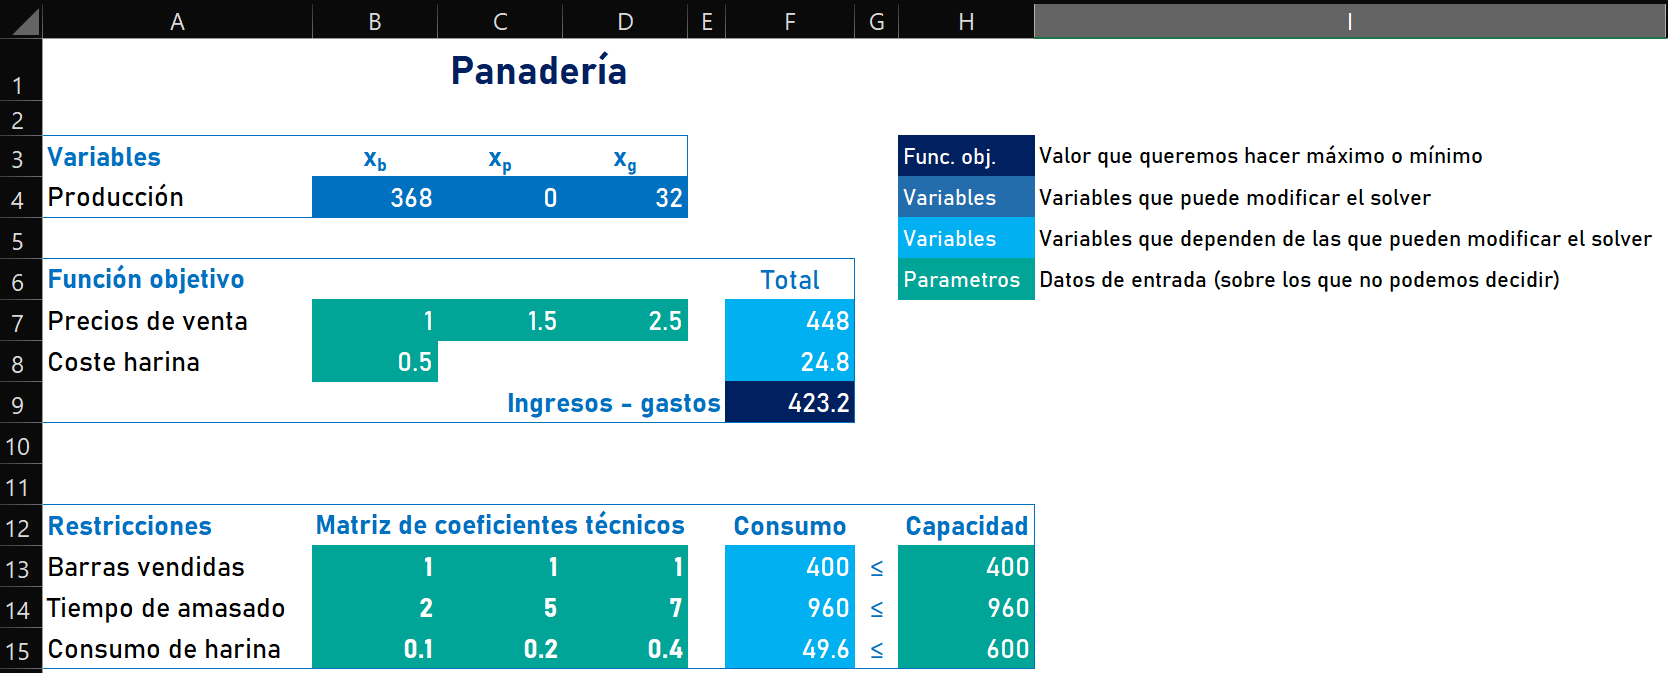
\includegraphics[width=10cm]{recursos/figs/panaderia/modelo_excel_panaderia.png}
\label{fig:model_excel_panaderia}
\end{figure}

Y la configuración del solver es la se muestra en la figura \ref{fig:solver_excel_panaderia}.

\begin{figure}[!h]
\caption{configuración del solver de Excel.}
\centering
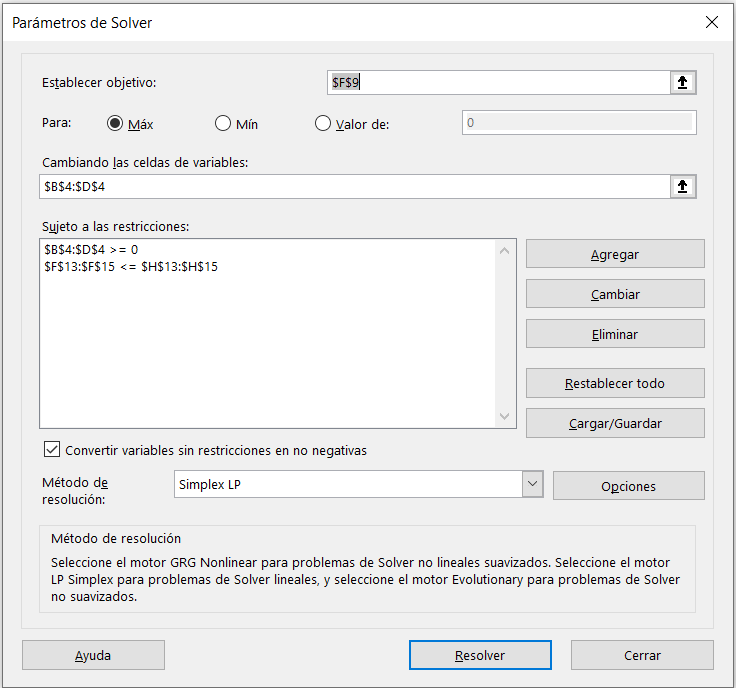
\includegraphics[width=10cm]{recursos/figs/panaderia/configuracion_solver_panaderia.png}
\label{fig:solver_excel_panaderia}
\end{figure}

La hoja de resultados que proporciona Excel es la de la figura \ref{fig:respuestas_excel_panaderia}. 

\begin{figure}[!h]
\caption{resultados (Excel).}
\centering
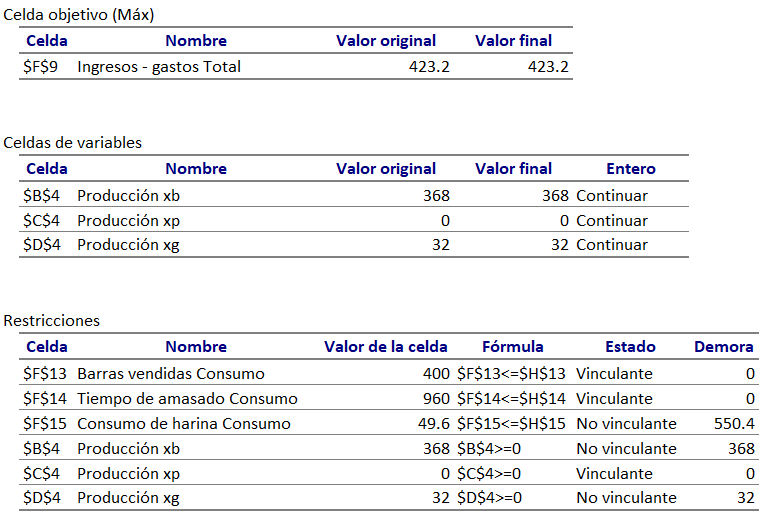
\includegraphics[width=10cm]{recursos/figs/panaderia/respuestas_excel_panaderia.png}
\label{fig:respuestas_excel_panaderia}
\end{figure}

La hoja de análisis de sensibilidad que proporciona Excel es la de la figura \ref{fig:model_excel_panaderia}. 

\begin{figure}[!h]
\caption{análisis de sensibilidad (Excel).}
\centering
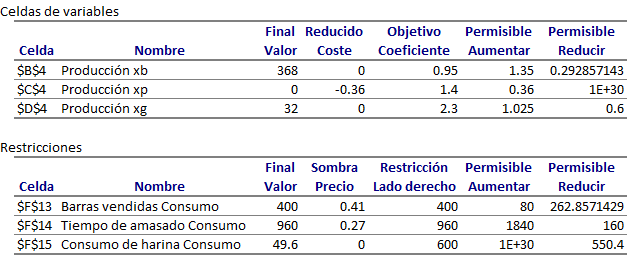
\includegraphics[width=10cm]{recursos/figs/panaderia/sensibilidad_excel_panaderia.png}
\label{fig:model_excel_panaderia}
\end{figure}

Los valores 1E+10 en Excel se refieren a $\infty$; Excel muestra el valor más grande que admite una fórmula en lugar de el símbolo de infinito.

\textbf{Modelo y resultados en Orstat}

El modelo en Excel se podría construir como el que se muestra en la figura \ref{fig:modelo_orstat_panaderia}.

\begin{figure}[!h]
\caption{modelo en Orstat.}
\centering
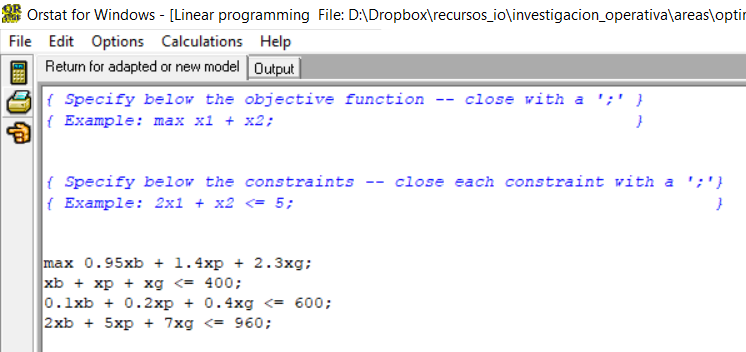
\includegraphics[width=10cm]{recursos/figs/panaderia/modelo_orstat_panaderia.png}
\label{fig:modelo_orstat_panaderia}
\end{figure}

El valor de la función objetivo, de las variables originales y de las holguras que ofrece Orstat se muestra en la figura \ref{fig:respuesta_orstat_panaderia}. Los costes reducidos que ofrece Orstat están cambiados de signo (los valores válidos son los de Excel o los de Orstat cambiados de signo).

\begin{figure}[!h]
\caption{resultado en Orstat.}
\centering
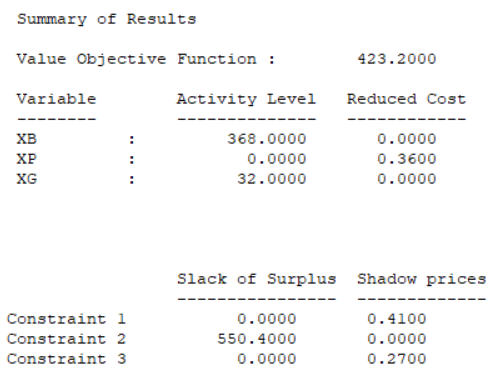
\includegraphics[width=10cm]{recursos/figs/panaderia/respuestas_orstat_panaderia.png}
\label{fig:respuesta_orstat_panaderia}
\end{figure}

Y la información relativa al análisis de sensiblidad de los coeficientes de la función objetivo del vector de disponibilidad de los recursos se muestra en la figura. 

\begin{figure}[!h]
\caption{análisis de sensibilidad en Orstat.}
\centering
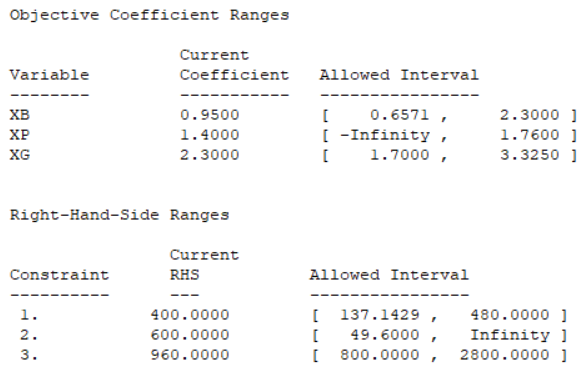
\includegraphics[width=10cm]{recursos/figs/panaderia/sensibilidad_orstat_panaderia.png}
\label{fig:sensibilidad_orstat_panaderia}
\end{figure}

\subsection{Análisis de resultados}

\textbf{Plan de producción y beneficio}

Los valores de las variables de la solución ótpima del modelo son:

\begin{equation}
\begin{split}
    x_b = 368\\
    x_c = 0\\
    x_g = 32\\
\end{split}    
\end{equation}

El plan de producción consiste en producir diariamente 368 baguetes, 32 de plan gallego y ninguna de pan de picos.

El beneficio de dicho plan de producción es 423.2 euros por día.

\textbf{Análisis de las restricciones}

Los valores de las variables de holgura ofrecen información sobre el uso de los recursos.

\begin{equation}
\begin{split}
    h_1 = 0\\
    h_2 = 0\\
    h_3 = 550.4\
\end{split}    
\end{equation}

La interpretación de los valores anteriores es la siguiente:
\begin{itemize}
    \item $h_1 = 0$: se vende una cantidad total de barras (de los tres tipos) exactamente igual al máximo que se pueden vender (400).
    \item $h_2 = 0$: se hace uso al completo del tiempo disponible para amasdo (960 minutos).
    \item $h_3 = 550.4$: no se consumen más que 49.6 kg con respecto a los 600 de los que se podría llegar a disponer.
\end{itemize}

Los valores de los precios sombra de las restricciones son los siguientes.

\begin{equation}
\begin{split}
    \pi_1 = 0.41\\
    \pi_2 = 0.27\\
    \pi_3 = 0\\
\end{split}    
\end{equation}

La interpretación de los valores anteriores es la siguiente:
\begin{itemize}
    \item $\pi_1 = 0.41$: si el máximo número de barras que se pudieran vender fuera de 401 (y no 400) el beneficio aumentaría en 0.41 euros.
    \item $\pi = 0.27$: si se dispusiera de un minuto más de amasado el beneficio aumentaría en 0.27 euros.
    \item $\pi = 0$: si se dispusiera de mayor cantidad de harina el beneficio sería el mismo (lógicamente, ya que en el plan de producción óptimo no se hace uso del total de la harina disponible).
\end{itemize}

Intervalos los coeficientes de las variables en la función objetivo

\begin{equation}
\begin{split}
    b_1 = [137.15, 480]\\
    b_2 = [800, 2800]\\
    b_3 = [49.6, \infty)\\
\end{split}    
\end{equation}

Orstat ofrece directamente los extremos de los intervalos. En el caso de $b_1$ los extremos 137.15 y 480 figura explícitamente en la tabla (figura \ref{fig:sensibilidad_orstat_panaderia2}).

\begin{figure}[!h]
\caption{análisis de sensibilidad (Excel).}
\centering
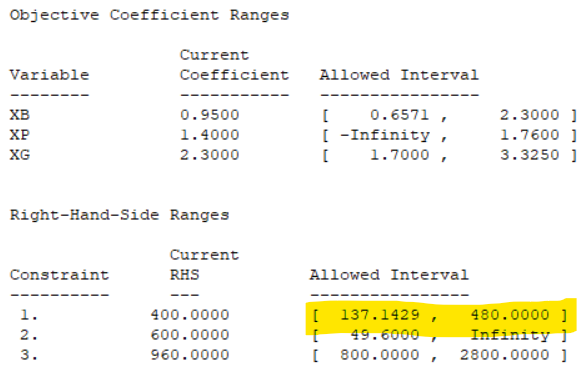
\includegraphics[width=10cm]{recursos/figs/panaderia/sensibilidad_orstat_panaderia2.png}
\label{fig:sensibilidad_orstat_panaderia2}
\end{figure}

En el caso de Excel, los extremos de los intervalos se obtienen a partir del valor original menos el valor "Permisible Reducir" para el extremo inferior y más el valor "Permisible Aumentar" para el extremo superior. En el caso de $b_1$, 137.5 se obtiene como 400 - 282.85 y 480 como 400 + 80 (figura \ref{fig:model_excel_panaderia2})

\begin{figure}[!h]
\caption{análisis de sensibilidad (Excel).}
\centering
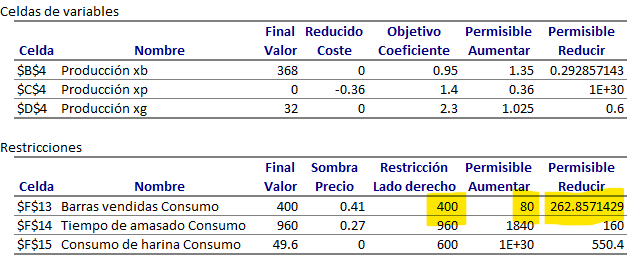
\includegraphics[width=10cm]{recursos/figs/panaderia/sensibilidad_excel_panaderia2.png}
\label{fig:model_excel_panaderia2}
\end{figure}



La interpretación de los valores anteriores es la siguiente:

\begin{itemize}
    \item $b_1 = [137.15, 480]$: la gama de productos que fabricaríamos (las actividades cuyas variables toman valor diferente de cero) serían las mismas siempre y cuando el límite total de barras vendidas no fuera menor que 137 ni mayor que 480. Para valores fuera de ese intervalo las variables diferentes de cero serían otras y la gama de productos del plan de producción óptimo sería otra.
    \item $b_2 = [800, 2800]$: la gama de productos que fabricaríamos (las actividades cuyas variables toman valor diferente de cero) serían las mismas siempre y cuando el tiempo de amasado disponible no sea menor que 800 ni mayor que 2800. Para valores fuera de ese intervalo las variables diferentes de cero serían otras y la gama de productos del plan de producción óptimo sería otra
    \item $b_3 = [49.6, \infty)$: la gama de productos no cambia siempre y cuando tengamos al menos 49.6 kg de harina disponibles cada día. Por debajo de ese valor, la gama de productos del plan óptimo de producción cambiaría.
\end{itemize}    


\textbf{Análisis de las variables (actividades)}

Los costes reducidos (criterios del simplex) son los siguientes:
\\
\\
\begin{equation}
\begin{split}
    V^B_b = 0\\
    V^B_p = -0.36\\
    V^B_g = 0\\
\end{split}    
\end{equation}

Para la única variable que es 0, $x_p$. su coste reducido indica el incremento de la función objetivo si esa variable tomar valor 1. Es decir, si decidiésemos fabricar una barra de pan de picos, el beneficio disminuiría en 0.36 euros.

El intevalo para los coeficientes de las variables es: 
\begin{equation}
\begin{split}
    c_b = [0.66, 2.3]\\
    c_p = (-\infty, 1.76]\\
    c_g = [1.7, 3.33]\\
\end{split}    
\end{equation}

La interpretación de los valores anteriores es la siguiente:
\begin{itemize}
    \item $c_b = [0.66, 2.3]$: mientras el beneficio untario de cada baguete esté entre 0.6 y 2.33 euros, la gama de productos no cambia, para valores fuera de este intervalo la gama cambia. Se puede comprobar que para valores menores, no interesará producir baguetes y para valores superiores a 2.3 interesará aumentar la cantidad de baguetes que se producen (más de los 368 actuales).
    \item $c_p = (-\infty, 1.76]$: mientras el beneficio untario de cada pan de pico sea menor que 1.76 euros, la gama de productos no cambia, para superiores el beneficio por barra de pan de picos sería suficiente como para que fuera ineteresante su producción. 
    \item $c_g = [1.7, 3.33]$: mientras el beneficio untario de cada pan gallego esté entre 1.7 y 3.33 euros, la gama de productos no cambia, para valores fuera de este intervalo la gama cambia. Se puede comprobar que para valores menores, no interesará fabricar pan gallego y para valores superiores a 3.33 interesará aumentar la producción de panes gallegos (con respecto al valor actual de 32).
\end{itemize}



